\documentclass[12pt,a4paper]{article}
%\documentclass[fleqn]{scrartcl}
\usepackage[english]{babel}
\usepackage{amsmath}
\usepackage{graphicx}
\usepackage{hyperref}
\usepackage{mathrsfs}  
%\usepackage[colorlinks=true,linkcolor=blue,urlcolor=blue,citecolor=blue,pdfusetitle]{hyperref}
\selectlanguage{english}
\usepackage{mathtools}
\DeclarePairedDelimiter\bra{\langle}{\rvert}
\DeclarePairedDelimiter\ket{\lvert}{\rangle}
\DeclarePairedDelimiterX\braket[2]{\langle}{\rangle}{#1 \delimsize\vert #2}
\usepackage{braket}
\usepackage{appendix}
\usepackage{ amssymb }
\usepackage{amsmath, amsthm}
%\usepackage[backend=biber,style=ieee,citestyle=numeric-comp, url=false, eprint=false, url=true, isbn=false, doi=false]{biblatex}
\usepackage[style=authoryear, backend=bibtex]{biblatex}
\usepackage{graphicx}
%\usepackage{biblatex}
%\usepackage[backend=bibtex]{biblatex}
%\bibliography{library.bib}
\addbibresource{bibli.bib}
\addbibresource{library.bib}
%\makeatletter
%\def\eqref{\@ifstar\@eqref\@@eqref}
%\def\@eqref#1{\textup{\tagform@{\ref*{#1}}}}
%\def\@@eqref#1{\textup{\tagform@{\ref{#1}}}}
%\makeatother 
\begin{document}
\begin{titlepage}
\begin{center}
\begin{figure}[h!]
\centering

\includegraphics[scale=0.3]{Bilder-für-text/uni-basel-logo-ogtag.png} 
\end{figure}

\noindent\rule{\textwidth}{1pt}
\Large\textbf{Fully quantum description of a three level maser, driven by a thermal bath}\\
\noindent\rule{\textwidth}{1pt}
\vspace{0.5cm}
\large{Master-Projekt}\\
%\large{nature12016}\\
\vspace{3cm}
%\normalsize{H. Bernien1, B. Hensen1, W. Pfaff1, G. Koolstra1, M. S. Blok1, L. Robledo1, T. H. Taminiau1, M. Markham2, D. J. Twitchen2,L. Childress3 R.Hanson}\\
\vspace{2cm}

\normalsize{ Sander Stammbach}\\
\normalsize{Prof. Patrick Plotts}\\
\vspace{0.2cm}
12 November 2022\\
\end{center}

\nopagebreak
\vspace{1cm}
\begin{minipage}{.25\textwidth}
 \begin{flushleft}
 \end{flushleft}
\end{minipage}
\hskip.4\textwidth
\begin{minipage}{.25\textwidth}
\end{minipage}
\end{titlepage}
\tableofcontents
\newpage
\section{Introduction}
One of the most important questions in thermodynamics is how to convert
thermal energy into work. For such tasks exists many classical engines, as
example the steam machines or gasoline engines. %To quantify heat-engines, it's common to look at the ergotropy.
In this master-project, a three level maser, driven by the coupling of a hot and a cold bath will get quantified .
The three-level maser is a Quantum heat engine (QHE). The work extraction from a classical heat engine is often a moving piston. But in this case
it is a driving field. In the year 1916 Albert Einstein, already discussed three ways of
light-matter-interaction (spontaneous emission, absorption, and stimulated
emission).\cite{Li2017}. \\In a paper from 1959.  Scovil and Schulz-DuBois investigated whether a laser is not
also a heat engine. In this paper, they take a maser as a device to transform heat into coherent radiation, because heat can make a population inversion. [\cite{Scovil1959}
In their thermodynamic analysis, they use a single-atom laser. They made a
groundwork for emerging theory of quantum thermodynamics. In practice and also for the calculations, two different reservoirs are necessary. The high-temperature reservoir can be
realized by a fast and accurate
estimation of the thermal occupation of propagating micro-
wave modes is highly desirable. \cite{Scigliuzzo2020}

\newpage

\section{System and model}
\subsection{3-level-Maser Model}
\begin{figure}[h!] 
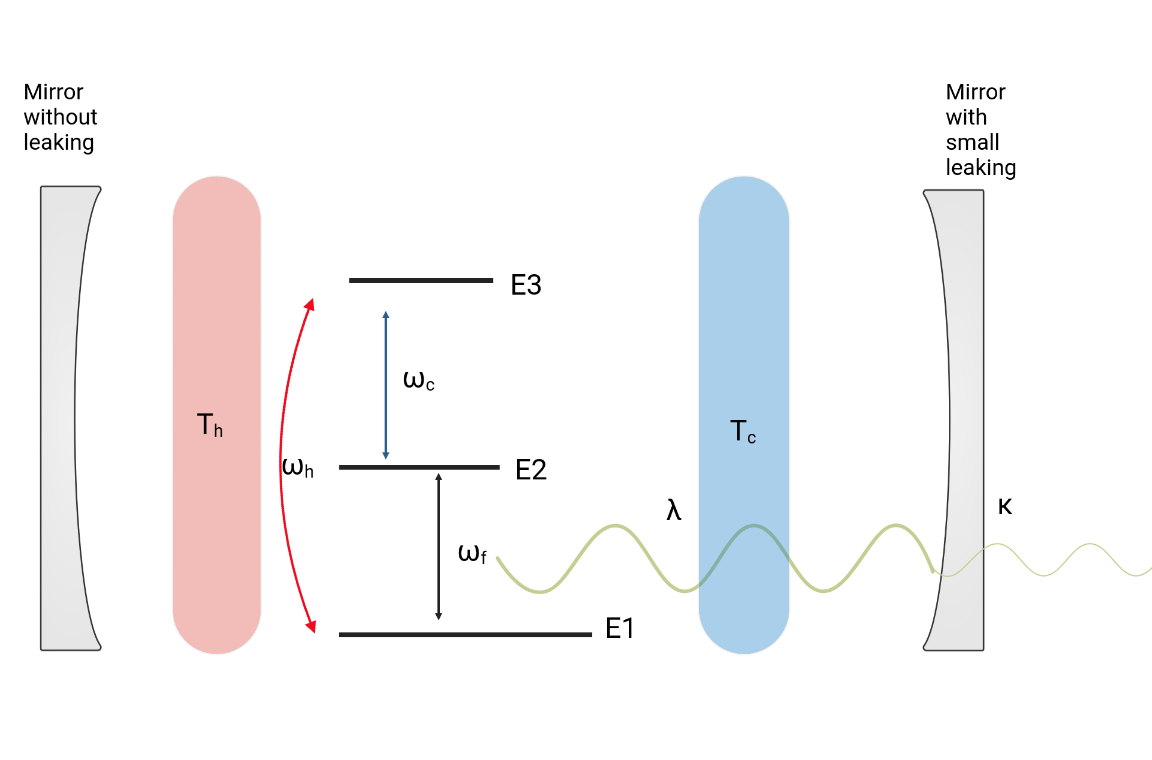
\includegraphics[scale=0.4]{Bilder-für-text/3-Level-System.png}
\caption{Schematic representation of a three-level maser heat engine
continuously coupled to two reservoirs of temperatures $T_h$ and
$T_c$. And the three energy levels $E_1,E_2,E_3$. The
system is interacting with a classical single mode field. $\lambda$
represents the strength of matter-field coupling.}
\end{figure}
A Maser/Laser consists of two elements. One of them is a gain medium and the other one is an optical resonator. A gain medium is always a material with an atomic transition between two atomic states. When an atom falls from an energetically higher state to an energetically lower state, a photon is created.
In a three level system the three energy levels are $E_1,E_2,E_3$ shown in Fig. 1.In a first part the system gets pumped from the lowest $E_1$ level to the highest level $ E_3$. The condition for the third level is that it falls to the middle level $ E_2$ very quickly. On average, the system is almost not in the third state. The resonator should then have a higher decay time, so that a population inversion can build up. This means that a particles is in the energetically higher state. From this state they come almost exclusively through stimulated emission into the lower state $ E_1$.  Our cavity is in  resonance, therefor we can set $\omega_{cav}=\omega_f$.
Emission is a necessary condition for coherent light. Coherent light means all the photons have the same phase and same frequency. \cite{Li2017}
Here we consider, the higher level will be reached with a interaction of a hot bath.  
We denote the frequencies of $\omega_h=(E_3-E_1)/\hbar$, $\omega_c=(E_2-E_1)/\hbar$ and $\omega_f=(E_2-E_1)/\hbar$
Interesting is that we get each thermal photon from the bath a lasing photon. 
The efficiency is given by the following formula:
\begin{equation}
\eta_{maser}=\frac{\omega_f}{\omega_h}<1-\frac{T_c}{T_h}.
\end{equation}

\subsection{Master-Equation} 
An arbitrary state on this the global Hilbert space of the system and the bath can be described by a total density operator $\rho_{tot}(t)$. %The total density operator can be written in the Hilbert space $ H_ {tot}= H_{system}+H_{bath}$. 
Encoded in this density 
operator is a complete description of the total system's state at a given time t. \cite{Li2017}. To derive the $\rho_{tot}$ we can solve a specific differential equation. This equation is called Lindblad-master-equation \eqref{1}. 
The Basic of this work is a three-level quantum system in a cavity. This three level system is driven by a hot and a cold bath. Those have the temperature $T_c$ and $T_h$. The cavity is build of two mirrors. One of the cavity have a small leaking, so that a small part of the photons can leave the cavity. This leaking is quantified by a constant $\kappa$.
In the calculation, the temperature of the thermal bath is constant, therefore 
it is possible to use the Lindblad-master equation. 
In this case the master equation is get solved for the steady states.
A steady state is a state or condition of a system or process, here the energy states of an atom, that the density matrix of the state does not change in time, or the changes are negligibly. Therefore all observables do not change in time either. 
It contains the whole description of the three-level system and the cavity.
In Fig.1 is shown a three-level system:
\newpage


The master equation is:
\begin{equation}
\dot{\rho}(t)=\frac{1}{i \hbar}[H,\rho]+ \mathcal{L}_{h}\rho+ \mathcal{L}_{c}\rho+ \mathcal{L}_{cav}\rho. \label{1}
\end{equation}
$H$ is the the Hamilton operator. The interaction with the various environmental heat baths is described by the Liouvillian $\mathcal{L}$. This $\mathcal{L}$ is also called superoperator. 
The first part of eq \eqref{1} is the von Neuman-equation,  the analogue of the Schrödinger equation but for density matrices. This part of the equation is unitary and therefore the process is reversible.
The non-unitary part of the equation $\mathcal{L}\rho$ include the superoperator $\mathcal{L}$, which act on the density operator.  A superoperator is a linear operator acting on a vector space of linear operators, as example a density operator.
$\mathcal{L}$ consist of three parts. $\mathcal{L}_h $ describe the interaction with the hot bath.
$\mathcal{L}_c$ is the contribution from the interaction with the cold bath coupled with the atom.
$\mathcal{L}_{cav}$ describe the photons which in the cavity. $\kappa$ is a parameter which describe the rate of photons which leave the cavity.
The Hamiltonian describes the energy. 
The atomic field system is composed of two crucial 
parts; the atomic states, the cavity field, and the interaction between the two.
The total Hamiltonian
\begin{equation}
H=H_{free}+H_{int}
\end{equation}
The total Hamiltonian consistof two parts. The part of the photons is, which describes the photons in the cavity:
\begin{equation}
H_{free}=\sum_{i=1}^3 \hbar \omega_i \ket{i}\bra{i}+\hbar \omega_f a^{\dag}a,\label{2}
\end{equation}
And the interaction Hamiltonian or Jaynes-Cummings Hamiltonian:
\begin{equation}
H_{int}=\hbar g(\sigma_{12}a^{\dag}+\sigma_{21}a).\label{3}
\end{equation}
The coupling constants $g$ strong for the Hamiltonian and the $\kappa$ for the Liouvillian part. 
The coupling constant $g$ is given by $\frac{\Omega}{\hbar}$.
\newpage
The interaction with the various environmental heat baths is described by the Liouvillian:
\begin{equation}
\begin{aligned}
\mathcal{L}\hat{\rho}=\frac{\gamma_h}{2}(n(\omega_h,T_h)+1)   \cdot \mathcal{D}[\sigma_{13}]\rho
+\frac{\gamma_h}{2}n(\omega_h,T_h)\cdot \mathcal{D}[\sigma_{31}]\rho \\
+\frac{\gamma_c}{2}(n(\omega_c,T_c)+1)\cdot \mathcal{D}[\sigma_{23}]\rho
+\frac{\gamma_c}{2}n(\omega_c,T_c) \cdot \mathcal{D}[\sigma_{32}]\rho \\
+\kappa((\omega_f,T_f)+1)	\cdot\mathcal{D}[a]\rho+
\kappa n(\omega_f,T_f)\cdot \mathcal{D}[a^{\dag}]\rho.
\end{aligned}
\end{equation}
The $\sigma_{12} $ is the transition operator and defined as $ \ket{1}\bra{2}$. Similar for $\sigma_{13}=\ket{1}\bra{3}, \sigma_{23}=\ket{2}\bra{3}=a$ . It describe the transition between a atomic state $a$ to $b$.
$\mathcal{D}$ is defined with following formula:
\begin{equation}
\mathcal{D}[A]\rho=(2A \rho	A^{\dag}-A^{\dag}A\rho-\rho A^{\dag}A),
\end{equation}

The Bose-Einstein occupation number. It is the mean number of excitations in the reservoir damping the oscillator  . It describes the mean occupation number $\langle n(E) \rangle$ of a quantum state of energy $E$, in thermodynamic equilibrium at absolute temperature $T $ for identical bosons as occupying particles. n depends on the temperature and the frequency.
$n$ is defined as:
$
n(\omega,T)=\frac{1}{\exp[\frac{\hbar \omega_i}{k_b T_i}]-1},
$
The  prefactor $\gamma_c ,\gamma_h$ describes the spontaneous decay rates and are in this calculation generally small.
The Liouvillian has different constants. 
\section{Methods}
\subsection{Software}
For the hole implementation of the tree-level-system in a cavity, I used qutip. Qutip is library in python, which allows to solve masterequation pretty easy.
Further calculation and methods was easily applied in python. 
\subsection{Implementation of the tree-level-system in qutip}
Qutip can be used to solve master equations. For that we have to define constants.  
In our case only $\omega_f$ interact with the light. 
The constants $\hbar $ and the Boltzmann factor $k_B$ are 1.
also defined as constants are the three different Bose Einstein occupation $n_h$, $n_c$ and $n_f$
The transition-operators $\sigma_{ab}$ are  made by following qutip implementation:\\ $\sigma_{}ab=tensor(\ket{a}\bra{b}\cdot I_{(nph)}"$.\\
In the same way I implemented also the other transition operators and 
vg and v1 are basisstates.  "nph" is the maximum of the photonnumber in the cavity. If I set my maximum photon number to 30, I get 90 x 90 matrices. 
The projectors are implemented similarly, but wit the matrix $\ket{a}\bra{a}$
With those its easy to construct the Hamiltoniens, $H_{free}$ and $H_{int}$, as in Eq. \eqref{2} , Eq . \eqref{3} 
To calculate the the density matrices for steady states we can also use a qutip function, call steadystate().
this function needs the total Hamiltonian and a list of the non-unitary operators as arguments.
We can we can construct this list as a multiplication of our transition-operators and the tree different Bose Einstein occupation numbers times the different $\gamma$-factors. 
As output of the function steady state we get the density-matrices for steady-states. \cite{Nation2022}
\section{Lasing transition}

\subsection{Wigner function and Phase-averaged coherent states (PHAV)}
The output of a laser is coherent light.
The quantum description of coherent light is a coherent state. The photon number distribution of coherent light is a Poisson distribution. The randomized phase of a coherent state doesn't change the photon-number distribution. \\

A Wigner function is a representation of a general quantum state of light.
The function describe the probability density in phase space.

\begin{equation}
w(x,p)=\frac{1}{2\pi \hbar}\int_{- \infty}^{\infty} d\xi e^{\frac{-i p \xi}{\hbar}}\bra{x+\frac{1}{2}\xi}\rho\ket{x-\frac{1}{2}\xi}.\label{4}
\end{equation}

The Wigner function from a coherent state itself is a Gaussian. But the Wigner function of a phase-average-state has a non-Gaussian Wigner function. 
The mathematical description of a  PHAV is the same as a normal coherent state but with a random phase. So we get a new term of $exp(i\pi\phi)$ in it. 
The normal coherent state $\ket{\alpha}$ could represented by following formula: \cite{Allevi2013}
\begin{equation}
\ket{\alpha}=e^{-1/2|\alpha|}\sum_{n=0}^{\infty}\frac{|\alpha|^n e^{in\phi}}{\sqrt{n!}} \ket{n},
\end{equation}
To get the phase average state will get reach with the integral around two $\pi$.
\begin{equation}
\rho_{PHAV}=\int_0 ^{2\pi}\frac{d\phi}{2\pi}\ket{\alpha}\bra{\alpha}=\sum_{n=0}^{\infty}p_{nn}\ket{n}\bra{n}.
\end{equation}
this is equal to:
\begin{equation}
\rho_{PHAV}= \sum_{n=0}^{\infty}\exp(-|\alpha|^2)\frac{|\alpha|^{2n}}{n!} \ket{n}\bra{n}.\label{11}
\end{equation}
The $\rho_{PHAV}$ from Eq. \eqref{11} implemented in python could visualised with a Fock and Wigner plot  Eq, shown in Fig \ref{21}

\begin{figure}[hbtp]
\centering
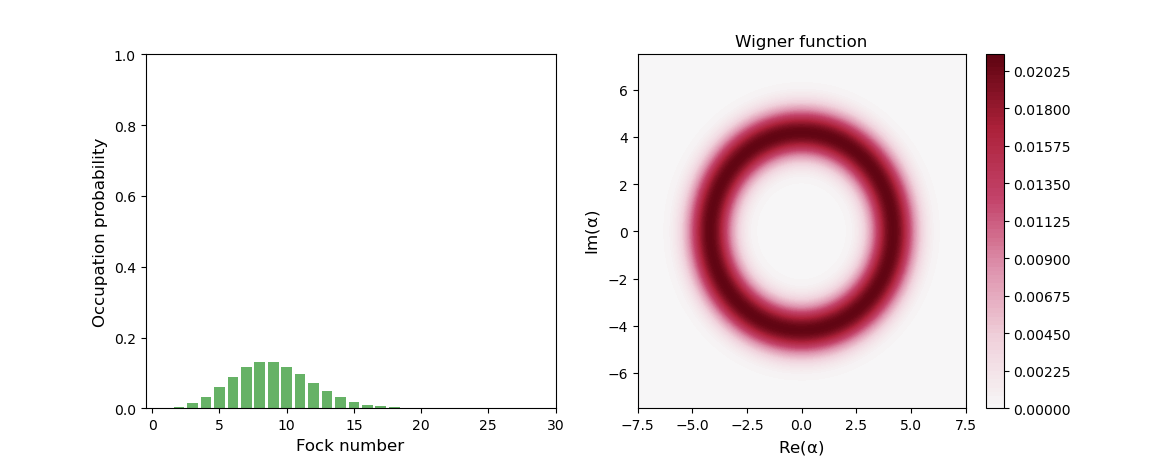
\includegraphics[scale=0.4]{Bilder-für-text/PHAV-rho.png}\label{21}
\caption{The Wigner-Fock plot of the density matrix of $\rho_{PHAV}$ wit the parameter $\alpha=3.5$.}
\end{figure}


For the Wigner function \eqref{4} we get finally following equation:
\begin{equation}
W(z)=2  \exp\bigl[-2\bigl(|\alpha|^2+|z|^2\bigr)\bigr) I_0 (4|\alpha| |z|).
\end{equation}
This function is plotted in Fig. 2
The consistent experimental and theoretical results we have obtained in the characterization of both PHAVs and their superpositions 2-PHAVs reinforce the
possibility of using them for applications to communication protocols. \cite{Allevi2013}
\begin{figure}[h!]
\centering
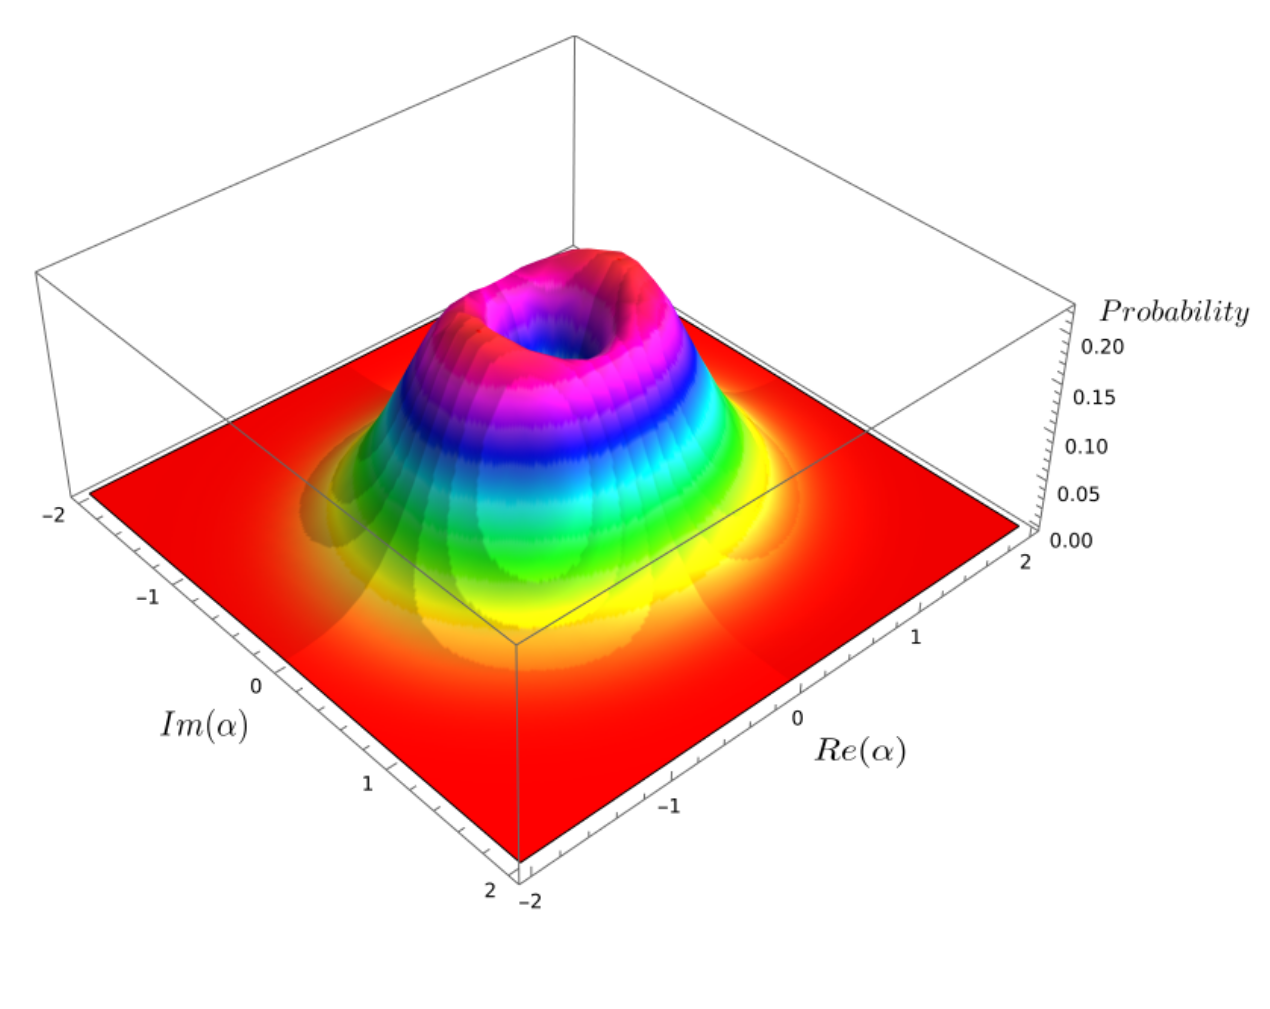
\includegraphics[scale=0.2]{Bilder-für-text/PHAV.png}
\caption{Plot of the Wigner function form a PHAV state}
\end{figure}

The first Result are Fockplots and Wigner-density-plots.
For all calculations, I set the parameters  $\hbar$ and $k_b$ equal to one. $\gamma_h, \gamma_c $ are set to $ 1$. And $\kappa=0.028$
I tested those with different set of parameters. 
shown in Fig. 3 and Fig. 5.\\
Those rings which are shown in Fig. 3 and Fig 5, are similar to the plot of Fig. 2
If we have a small $\kappa$ means less photons will not leave and stay in the cavity. we see that in the Fockplott.
In the first plot I set a high leaking-parameter $\kappa=1$. Shown in Fig. 3
This means that many photons leave the cavity, and only a few remain in the cavity. 
We see, that the occupation-number in the fock-plot is most zero and the probability for one photon is just 0.1.

\begin{figure}[hbtp]
\centering
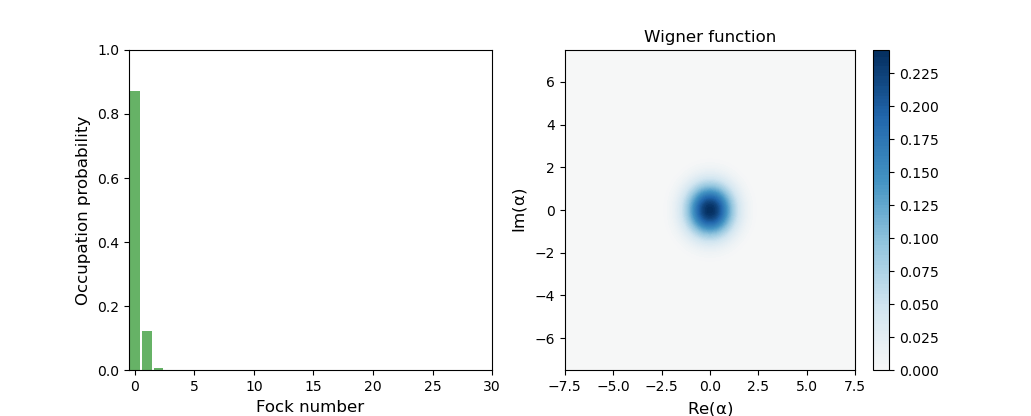
\includegraphics[scale=0.4]{Bilder-für-text/Figure_1.png}
\caption{The parameters for the first plot are$ n_h=2.6 n_c=0.001 n_f=0.02,\kappa=1$. The temperature for the warm bath is 460. Cavity with a big leaking}
\end{figure}\newpage

In the second plot I took the same parameters again, but with a lower $\kappa$. We get a better distribution in the Fockplot and a PHAV state in the Wigner function. 


\subsection{Double threshold behaviour}
If the lasing gain decreases when $T_h$ is too high, and this system shows a double threshold behaviour: when the hot bath temperature $T_h$ is
too low $(T_h \approx T_c)$, the excitation is too weak and the system
is below the lasing threshold; with the increasing of $T_h$ further, population inversion happens and the lasing light comes out. But when $T_h$ keeps increasing, then the lasing gain starts to decrease again and goes below the threshold. This is another critical point, after which the output light becomes thermal radiation again.
To avoid this double threshold behaviour, we study a three-level system.
This double threshold behaviour can perhaps described by the zeno effect.

\begin{figure}[h!]

\hspace{-1cm}
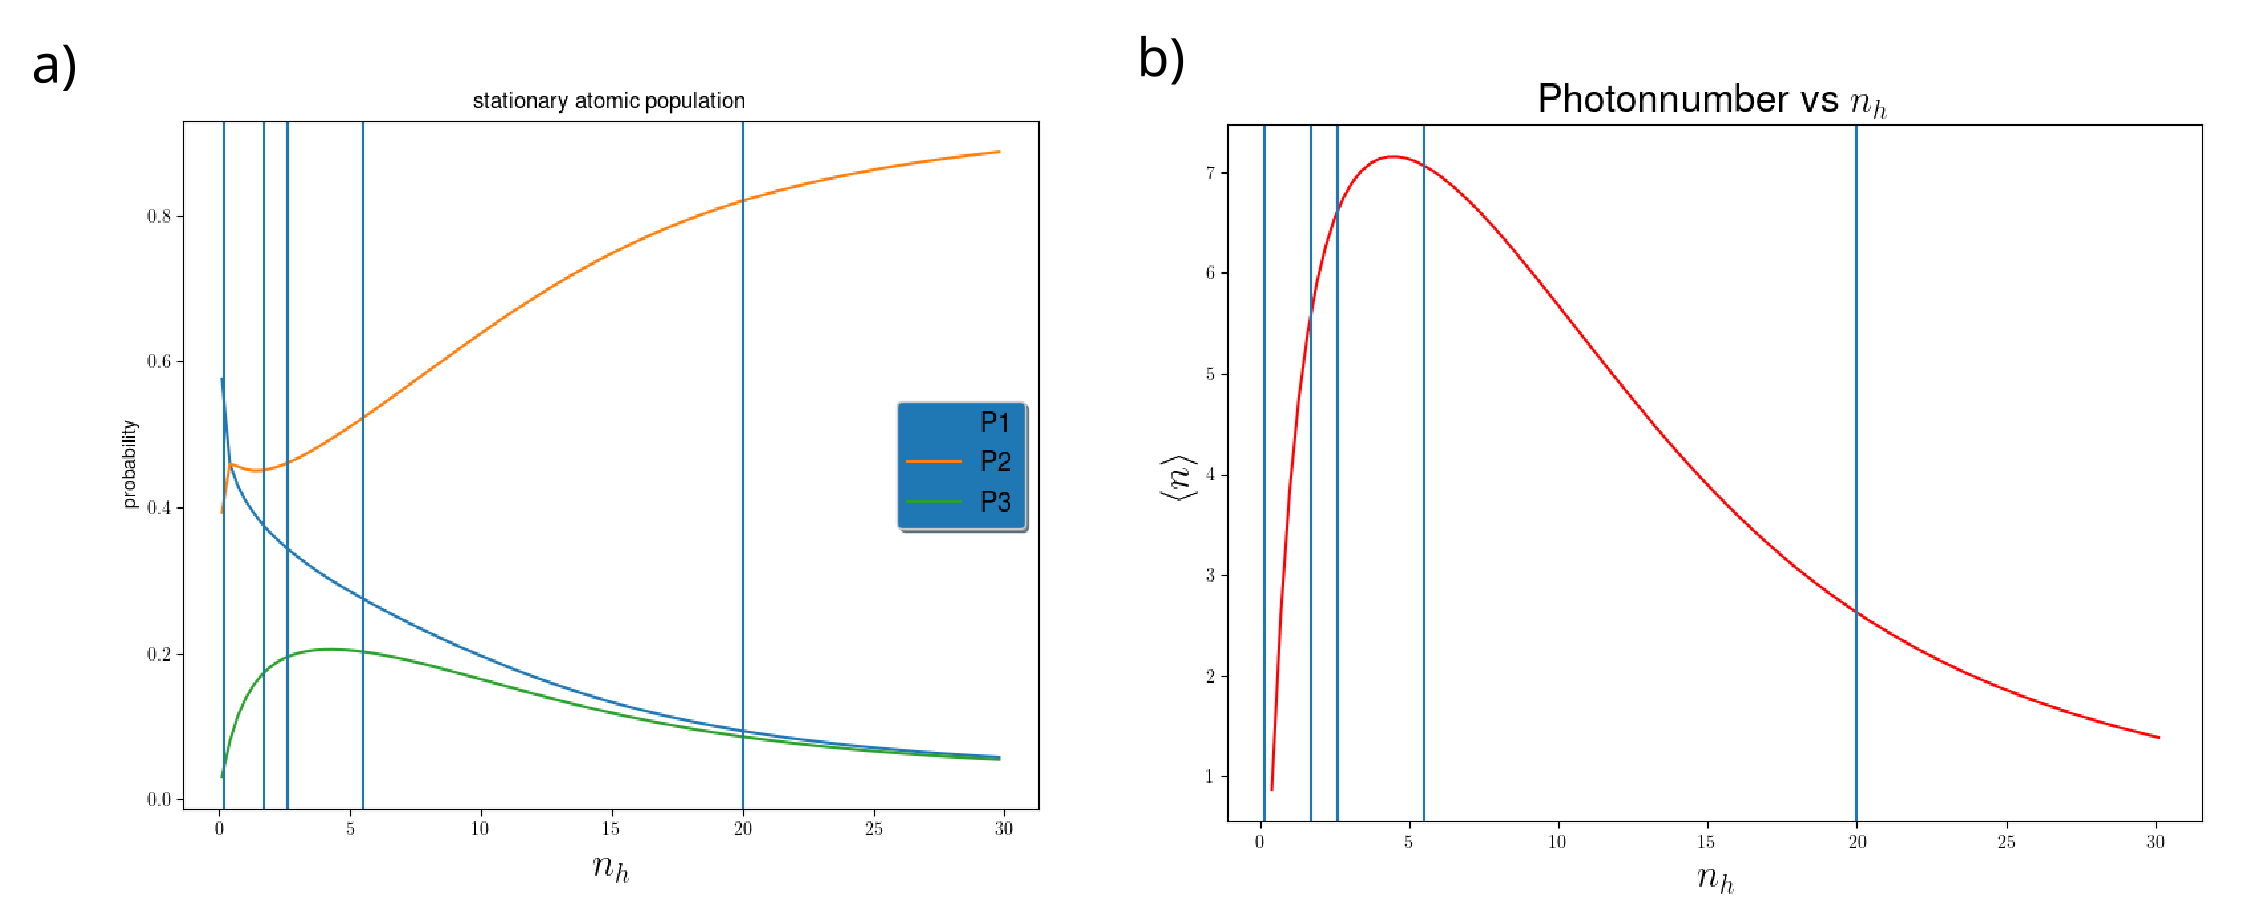
\includegraphics[scale=0.2]{Bilder-für-text/Energy_1.png}
\caption{In Fig. 4a the probability for a atom to sty in a state 0, 1 or 3 vs $n_h$ with the parameters The parameters for the first plot are $n_c=2.6 ,n_f=0.02,\kappa=0.01 $ and $n_h$ is from $0-30$ the blue lines marks the the values for $ n_h$ for which the Wigner functions are plotted. In Fig. 4b we see, the the expectation value of the photon number versus different $n_h$ }
\end{figure}

In a first step the reduce density matrices $\rho_{free}$ will be used to make Wigner and Fock plots.
Because $\rho=\rho_{system}\otimes \rho_{bath}$, It is possible to make the partial trace of $\rho$ with qutip, to trace out the reduced density matrices $\rho_{free}$. The Fock plot and the Wigner plot is also done with a qutip function.\\
\ \newpage
\ \newpage
\begin{figure}[h!]
\hspace{-0cm}
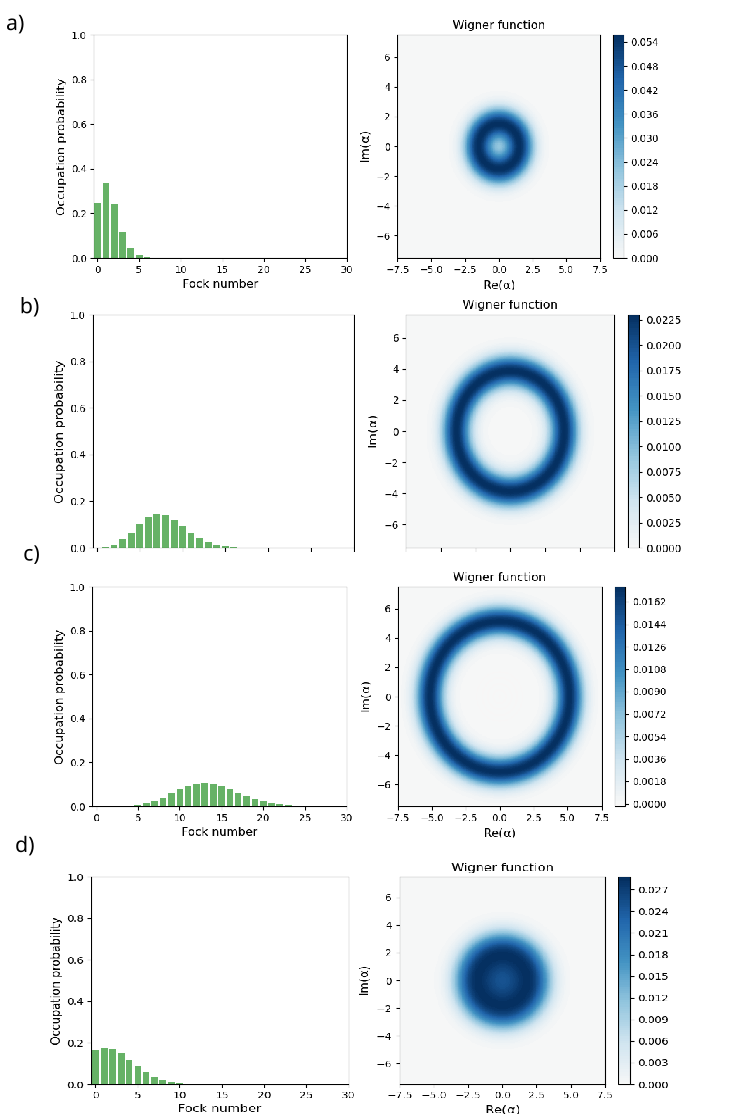
\includegraphics[scale=0.55]{Bilder-für-text/4-fits2.png}
\caption{For all of the four fits the parameters are $n_c=0.001 n_f=0.02,\kappa=0.1$ just the parameter for $n_h$ Cavity with a small leaking.
\textbf{a)}The parameters for $n_h$is $n_h=0.2 $.
\textbf{b)}$ n_h=2.6$ 
\textbf{c)} $ n_h=5.5$ 
\textbf{d)}$ n_h=20$. 
}
\end{figure}
\ \newpage
We see in in Fig 5a that start to get a PHAV
If we increase  $20>n_h >>0.2 $,
then the cavity photon number increase again when increasing $n_h$ at the very
high temperature regime, as shown in Fig. 5b, Fig 5c . This is because,
in this regime, the population has been almost inverted
thus the increase of the hot bath temperature $T_h$
can no longer bring in a significant increase to the photons gain.
The hot bath no longer has
any weakening effect to the lasing, thus more lasing photons
can be produced in the cavity, and the lasing power can be
increased. But, still, the cavity photon number is limited due to
the single atom feature.
If we further increase  $n_h >10$, we see the double threshold behaviour. 
In Fig. 5d we get by $n_h=20$ a thermal state.
%(Dieser Abschnitt ist zum teil übernommen und muss noch umgeeschrieben werden)
\section{Thermodynamics}
\subsection{Heat currents}

 When we work with density matrices, its common to work with expectation values with $\langle A \rangle=Tr[A\dot{\rho}]$.
 $A$ is a operator and describe a measurement.
With this we can calculate the expectation value from an Operator. 
To calculate the expected heat flow we can take the partial trace from 
\begin{equation}
\langle J\rangle=Tr[H_{free}\cdot \mathcal{L}_h[\rho]]+Tr[H_{free}\cdot \mathcal{L}_c[\rho]]+Tr[H_{free}\cdot \mathcal{L}_{cav}[\rho]].\label{13}
\end{equation}
A part of my work is to calculate the occupation number analytically. 
The calculation is made in two steps. for the warm and the cold bath, we have a transition-operators in the trace.
The trick of this calculation is, to get the form $Tr[\sigma_{ab}\rho \sigma_{ab}^{\dag{}}]$ because this correspond to the probability that the system is in state b $(Pb)$
The equation gave the following result:
\begin{equation}
\langle J_h \rangle=Tr[H_{free}\cdot \mathcal{L}_h[\rho]]=\hbar \omega_h \gamma_h (2n_h+1) \cdot( P1-P3) ,
\end{equation}
The same calculation can be done for the interaction with the cold bath.
\begin{equation}
\langle J_c \rangle=Tr[H_{free}\cdot \mathcal{L}_h[\rho]]=\hbar \omega_h \gamma_h (2n_c+1) \cdot( P2-P3) ,
\end{equation}
For the calculation the $Tr[H_{free}\cdot \mathcal{L}_{cav}]$, I get the following result:
\begin{equation}
\langle J_{cav}\rangle=T[H_{free}\cdot \mathcal{L}_{cav}[\rho]]=2\hbar \omega_{cav}\kappa (n_{cav}-\langle a^{\dag{}}a \rangle).
\end{equation}

with the density matrix times the $L_{p}\rho$ i calculated on the heat flux by taking the trace of $H \mathcal{L}\cdot \rho$. 
and plot this for 200 different  $g$ `s 
so the goal of this work is to find Einstein-Bose-distributions which yield a PHAV state.
as in the paper \cite{Allevi2013} 

In the second step of the calculation of the  expectation value from energy flow depends on different coupling constants $g$.
In other words I plotted the Trace from the density matrices times the Liouvilian against the coupling constant.
The master equation depends on three different Liovillien therms. I calculated the expected heat flow for every different interaction. the cold interaction the warm and the interaction with the cavity
The figure 6 shows  for the parameters $n_h=n_c=2.6 n_f=0.02,\kappa=0.01 $ is shown below.

\begin{figure}[hbtp]
\centering
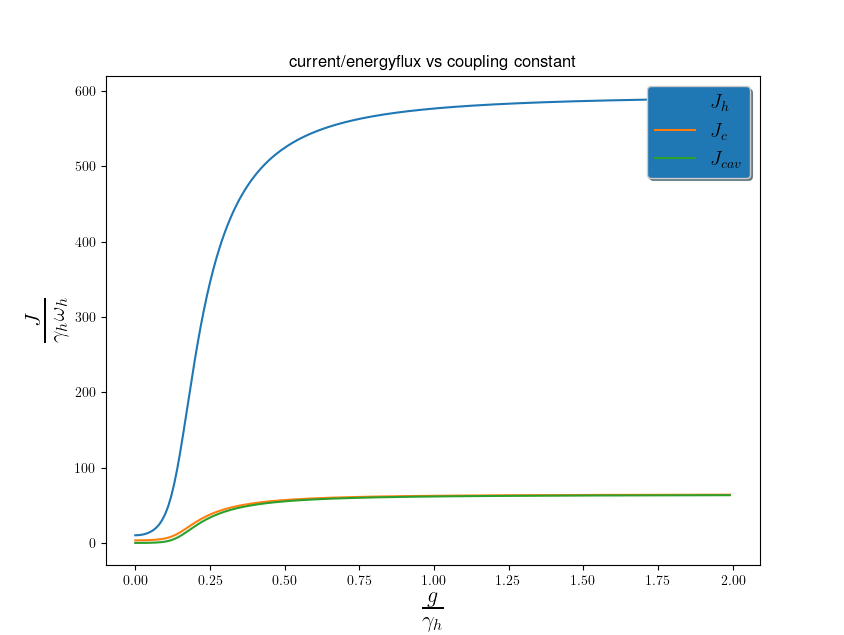
\includegraphics[scale=0.6]{Bilder-für-text/Energie_1.png}
\caption{Energy flux vs g with the parameters The parameters for the first plot are $ n_h=2.6,n_c= n_f=0.02,\kappa=0.01 $}
\end{figure}

\newpage
\subsection{Entropy production}
A other useful scientific concept is the entropy. its also a physical physical property. 
The entropy production is given by the formula\\ $\dot{\sigma} =\frac{J(n_h)}{T(n_c)}+\frac{J(n_c)}{T(n_h)}+\frac{J(n_{cav})}{T(n_{cav})}$.
As already seen in Fig. 4b we have a optimum parameter $n_h$.  in Fig. 4a we see the probability for $P1,P2,P3$ is in the region of $n_h=5 $ well distributed. We see alsou that  this correspond with the average of the photon number.
The higher the entropy, the more the state of the three-level system changes and the more photons are emitted.
We see that the entropy production correlate with the average of photon number in Fig 4b
\begin{figure}[hbtp]
\centering
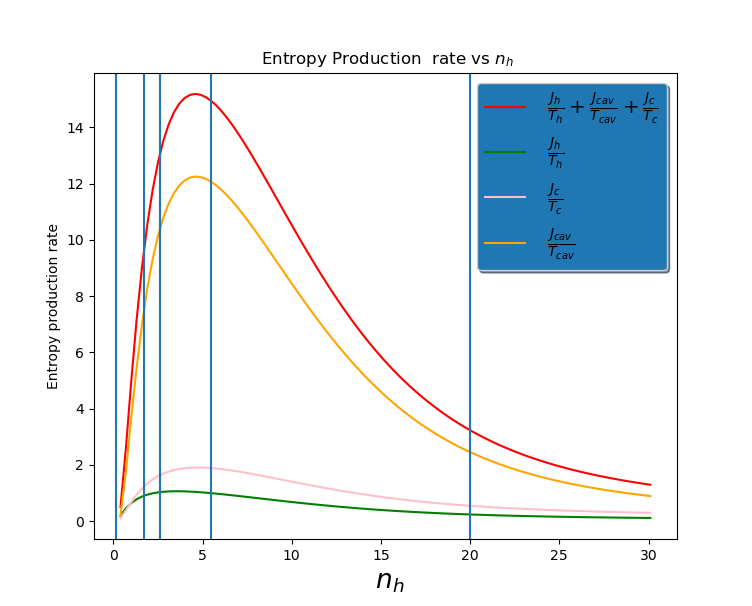
\includegraphics[scale=0.6]{Bilder-für-text/Entropy}
\caption{The entropy production for different $n_h$.The parameters for the first plot are$n_c=0.001 n_f=0.02,\kappa=1$. As in paper \cite{Li2017} is used the values for the frequencies $\omega_f=30\frac{1}{t},\omega_h=150\frac{1}{t}, \omega_c=120\frac{1}{t}$.}
\end{figure}



\newpage
\section{Conclusion an d outlook}
With the condition that $n_c, n_{cav}$ is almost zero, the leaking $\kappa$ is small too, and the hot bath have a value between 1 and 5.5 When we compare the Winger functions of the numerical calculated states with the Wigner plot of a PHAV state Fig. 4a, we see, that pretty similar. As conclusion; it's possible to get a phase average coherent state. 
In Fig. 6 we see the average of the current, calculated with the formula Eq. \eqref{13} For different coupling constants, $g$
we see, that the current increase at most between the $ 0<g<0.25$ 
In Fig. 4a we see the probability in which state an atom is. If we increase the temperature from the hot bath, we see that the occupation probability of $P2$ increase as well. However, the probability of an atom being in the $P1$ or $P3$ state decreases with increasing $n_h$. The probability of $P1$ and $P2$ is thus inversely proportional to the temperature.
The problem is that the cycle of photons can be stopped, because the probability that the photons goes from the ground state into the highest state is too small.
Fig. 4a is consistent with the Wigner plots.
The Fig. 4b helps to get some conclusion about, when the system start to lasing and when it stops. With a too small temperature, It has not enough energy in the system and to have photons in the upper band. If $n_h$ change property, a maximum get reached. If the temperature increasing further, the system is in the highest level,therefore the Rabi oscillation between the 0 and the $E_2$ doesn't exist any more.
At higher heat of the warm bath, dephasing of the system occurs. Thus, it interacts more with the environment. This has the same effect as if the system is measured often. The Zeno effect then shows that the system no longer oscillates between two different states. Also, spontaneous  emission could be a problem, that the photons which leave the atoms are not in a coherent state anymore. \cite{Niedenzu2019}
\cite{Scovil1959}
%\section{References}
\printbibliography



\newpage
\section{Appendix}
The hole Master equation without any substitution:
\begin{equation}
\mathcal{L}\hat{\rho}=\frac{\gamma_h}{2}\biggl[  \frac{1}{\exp[\frac{\hbar \omega_h}{k_b T_h}]-1}+1   \biggr]\cdot \biggl(2 \sigma_{13}\cdot\rho\cdot \sigma_{13}^{\dag}-\sigma_{13}^{\dag}\sigma_{13}\rho-\rho\sigma_{13}^{\dag}\sigma_{13}\biggr) $$\\$$
+\frac{\gamma_h}{2}\bigg[  \frac{1}{\exp[\frac{\hbar \omega_h}{k_b T_H}]-1}\biggr] \cdot\biggl( 2 \sigma_{31}\cdot\rho\cdot \sigma_{31}^{\dag} -\sigma_{31}^{\dag}\sigma_{31}\rho-\rho\sigma_{31}^{\dag}\sigma_{31}\biggr)$$\\$$
+\frac{\gamma_c}{2}\biggl[  \frac{1}{\exp[\frac{\hbar \omega_c}{k_b T_c}]-1}+1   \biggr]\cdot \biggl(2 \sigma_{23}\cdot\rho\cdot \sigma_{23}^{\dag}-\delta_{23}^{\dag}\sigma_{23}\rho-\rho\sigma_{23}^{\dag}\sigma_{23}\biggr)$$\\$$
+\frac{\gamma_c}{2}\bigg[  \frac{1}{\exp[\frac{\hbar \omega_c}{k_b T_c}]-1}\biggr]
\cdot\biggl( 2 \sigma_{32}\cdot\rho\cdot \sigma_{32}^{\dag}-\sigma_{32}^{\dag}\sigma_{32}\rho-\rho\sigma_{32}^{\dag}\sigma_{32} \biggr)$$\\$$
+\kappa\biggl[ \frac{1}{\exp[\frac{\hbar w_f}{k_b T_f}]-1}+1\biggr] \cdot\biggl( 2 a\rho a^{\dag} -a^{\dag}a\rho-\rho a^{\dag}a\biggr)$$\\$$
+\kappa\biggl[ \frac{1}{\exp[\frac{\hbar w_f}{k_b T_f}]-1}\biggr]\cdot \biggl(2 a^{\dag}\rho a -aa^{\dag}\rho-\rho a a^{\dag}\biggr)$$\\$$
\end{equation}


\begin{figure}[hbtp]
\caption{.}
\centering
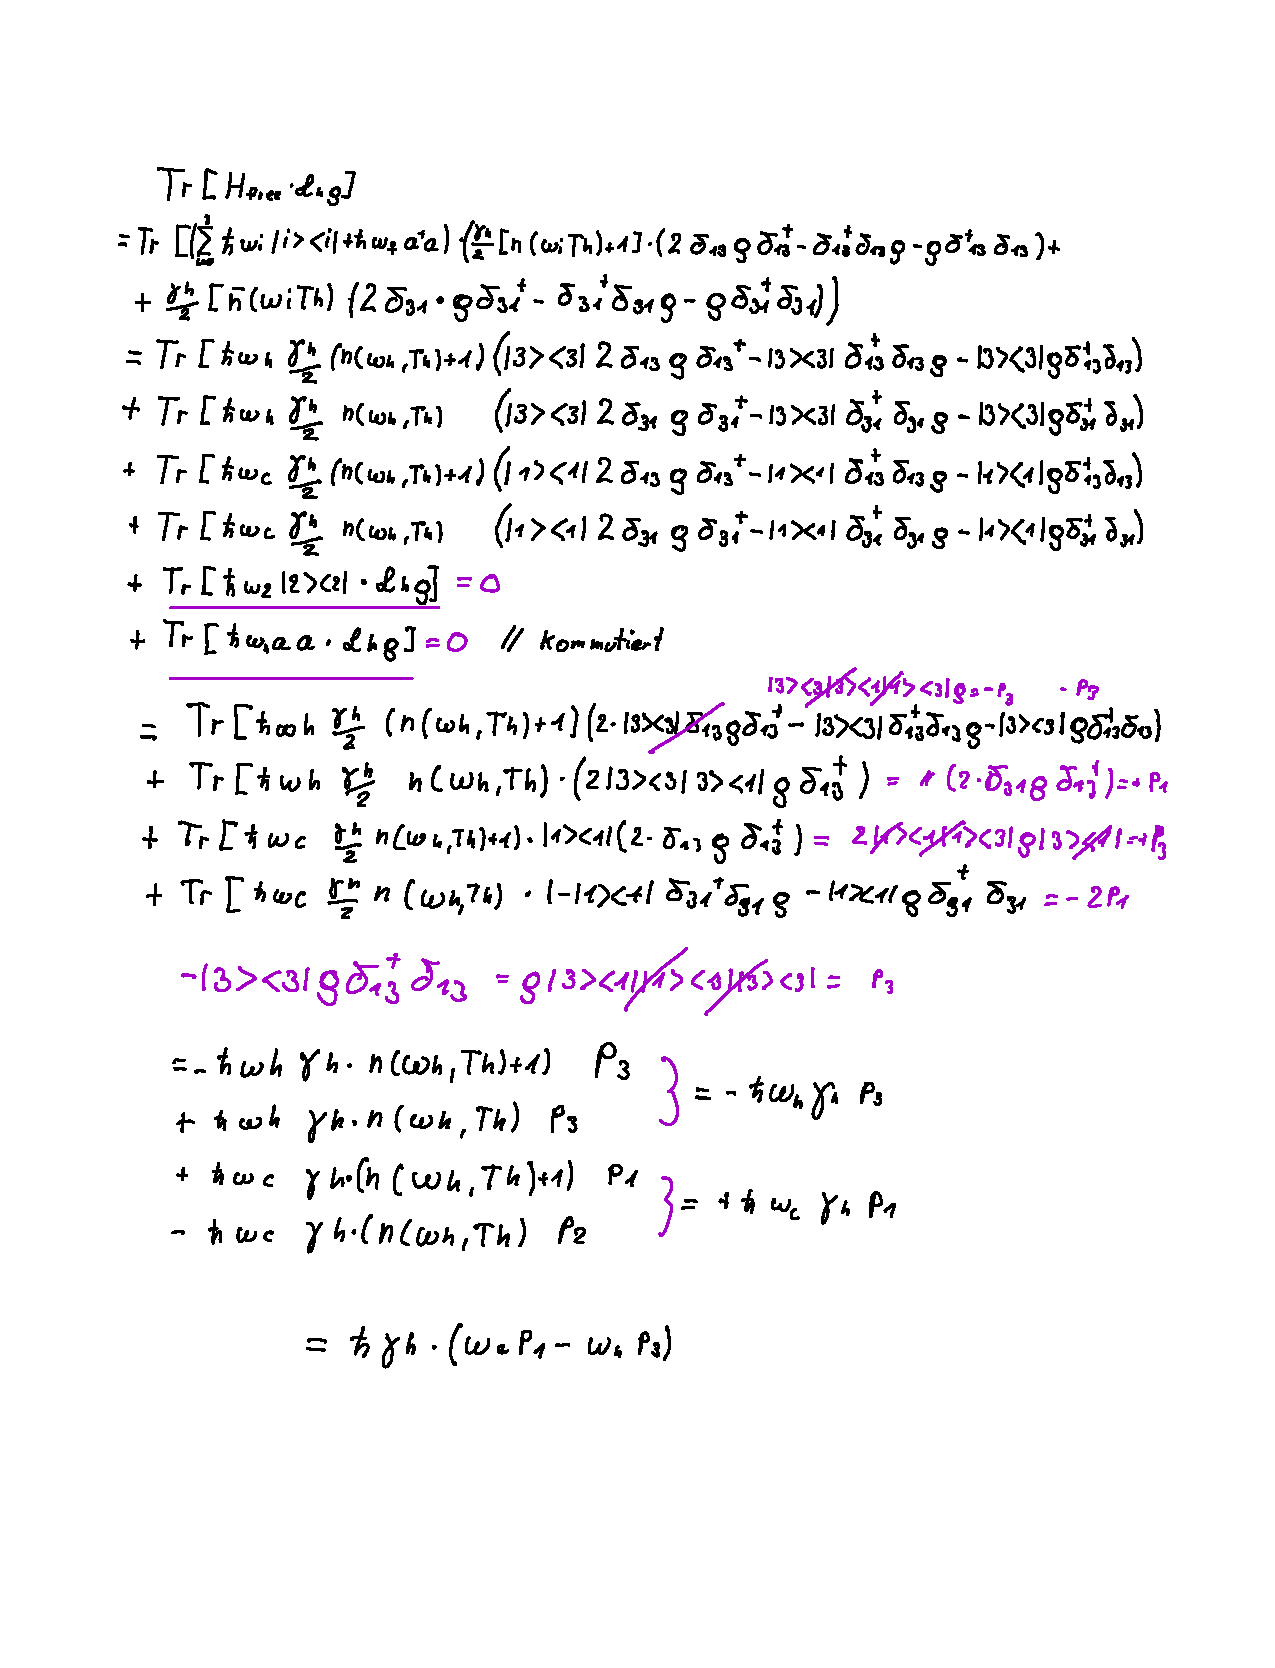
\includegraphics[scale=0.5]{Bilder-für-text/Berechnung-Tr[HL].pdf}
\end{figure}

\begin{figure}[hbtp]
\caption{.}
\centering
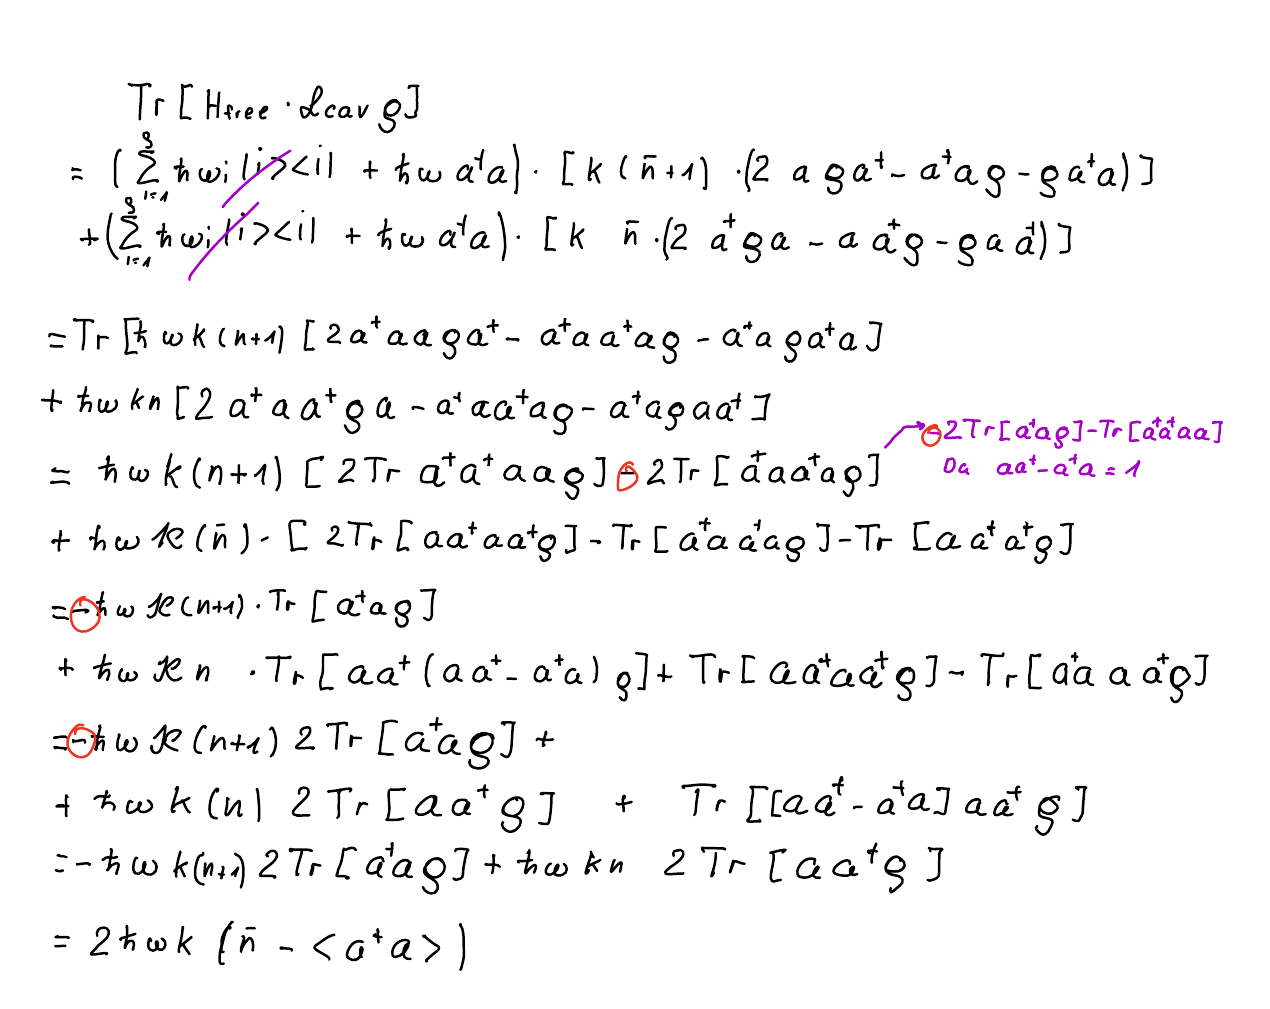
\includegraphics[scale=0.3]{Bilder-für-text/Berechnung-Tr[HL]2.png}
\end{figure}



\end{document}